%!TEX root = Main.tex
\documentclass[Main]{subfiles}

\begin{document}

\section{Hardware} % (fold)
\label{sec:hardware}

	\subsection{Platform} % (fold)
	\label{sub:platform}

		The processing platform chosen for this projet is a Xilinx Zynq-7000 All Programmable System on a Chip (SoC).
		The SoC (see Figure \ref{fig:ZynqArch}) features both a Processing System (PS) consisting of 650 MHz dual core ARM\textregistered{} Cortex A9 CPU with dedicated I/O and Memory and extensible FPGA Programmable Logic (PL) for HW synthesis.

		This enables the construction of a system with software, written in C++, running on the CPU, and with dedicated hardware for acceleration of computation and I/O handling.
		\begin{figure}[H]
			\centering
			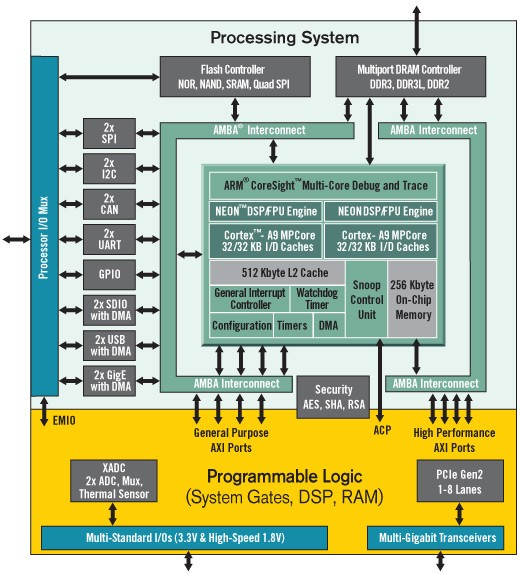
\includegraphics[width=0.5\linewidth]{ZynqArch}
			\caption{Zynq 7000-SoC Diagram}
			\label{fig:ZynqArch}
		\end{figure}

		
	
		% subsection platform (end)

	\subsection{Power} % (fold)
	\label{sub:power}
	
	% subsection power (end)

	\subsection{Sensors} % (fold)
	\label{sub:sensor}
	
	% subsection sensor (end)

	\subsection{Motor Control} % (fold)
	\label{sub:motor_control}
	
	% subsection motor_control (end)


% section hardware (end)

\end{document}